\documentclass[twocolumn,amsmath,amssymb,pra, floatfix]{revtex4-2}
\usepackage[utf8]{inputenc}
\usepackage{graphicx}
\graphicspath{ {figures/} }
\usepackage{siunitx}
\usepackage{hyperref}
\usepackage{float}

\begin{document}

\title{Physics 360-0: Brownian Motion}

\author{Jun Sung, Maura Lally}

\date{06-08-21}

\begin{abstract}
The purpose of this lab is to observe the Brownian motion of silica beads (of various diameters) suspended in water and measure the diffusion and Boltzmann constant. To achieve this, we view these beads under a microscope and use particle-tracking software to measure the mean-squared displacement of these beads over a period of time. We then use a simple model from statistical mechanics that gives us a relation between the diffusion constant and the mean-squared displacement. From this relation, we can extract both the diffusion and Boltzmann constants. Furthermore, we analyze whether changes to the bead density, frame rate, and track length have any noticeable effects on calculating the two constants. We find that we are generally successful in recovering the expected Boltzmann constant $k_B$: The majority of our results were within $2\sigma$ of the established value of $k_B$. Generally, our results were closest to the expected value when using a $1 \si{\mu m}$ sample at any dilution, with a frame rate of 10 and a track length of 15 or shorter.
\end{abstract}

\maketitle

\section{Introduction}
Consider a particle is suspended in a fluid (either liquid or gas). If we place ourselves in the shoes of this particle, then we see that we would be constantly bombarded from all sides by the constituents of the fluid. This bombardment results in the random motion of the particle, and we refer to such motion as Brownian motion.

Some might question why such a motion is important enough to be named, to which we would reply that it provided some of the first evidence of atoms. Furthermore, if one looks close enough, then they would find Brownian motion to exist in nearly every aspect of our lives (although it does not affect the macro world much, if at all).

In terms of how Brownian motion could be explained, Einstein published a paper in 1905 doing exactly that by showing that Brownian motion could be explained by assuming that fluids were composed of atoms moving randomly with an average kinetic energy.

For this lab, we will observe the Brownian motion of silica beads suspended in water and use particle-tracking software to measure the mean-squared displacement of these beads over a period of time. We then use a simple model from statistical mechanics to look at how diffusion scales with particle size.

\subsection{Brief Overview of Methods}
This lab will consist of one main experiment along with a few extensions. Starting with the main experiment, we will use the microscope and camera to record a 300-frame video of a slide with a drop of silica beads suspended in water. We then analyze the bead motion it captured via \texttt{TrackPy} and calculate the diffusion coefficient (as well as $k_{B}$). This process will be done for several particle sizes.

As for the extensions, we will look into how particle density (the concentration of the water drop), video frame rate (how many frames per second are captured by the camera), and track length (the minimum length that particle tracks must be in order to be included in the final analysis) affects the diffusion constant and the way that we analyze our data (e.g. we might adjust other parameters in \texttt{TrackPy} differently in order to obtain a result).

\subsection{Applications}
One area where Brownian motion can be applied (that might be a surprise to some) would be in finance. The stock market (and other markets in general) is assumed to follow Brownian motion \cite{econ}. In fact, the models used to describe Brownian motion are used to model financial asset and derivative pricing, which can further be used for risk analysis. 

Brownian motion is also applied in nanotechnology. As stated earlier, Brownian motion has little to no effect in the macro world. However, when we are dealing with the micro world, the effects of Brownian motion can no longer be ignored. In fact, it turns out that Brownian motion is one of the main controlling factors in the the realm of nanotechnology \cite{nano}. For example, the fluid can exert forces on a nano-machine that could potentially cause it's parts to stick together. Furthermore, the Brownian motion that a nano-machine undergoes could make it hard to control it's movement, which could impede the machine from doing what it was designed to do. 

\section{Theory}
As noted in the lab manual, the theory of Brownian motion of spherical particles can be derived from statistical mechanics. In particular, the velocities of small particles suspended in a fluid due to collisions with molecules obey a Maxwellian velocity distribution. We will follow the steps outlined in \cite{doi:10.1119/1.2386163} to derive the diffusion constant $D$ in terms of the fundamental parameters of the particles and liquid. Because Brownian trajectories are continuous, random, and irregular, it would be hard for us to work with the data as-is. However, we can work instead with the mean-squared displacement for each trajectory. 

\subsection{Mean-Squared Displacement Derivation}
We start by introducing the Langevin equation of a particle which has mass $m$ and velocity $v$:
\begin{equation}
    m \frac{ d v }{ d t }
    =
    - \alpha v + F( t ) 
    \label{eq:theory-1}
\end{equation}
where $\alpha$ refers to the dampening constant and $F( t )$ is a random fluctuating force due to molecular collisions. Furthermore, if this particle is a sphere, then $\alpha$ is given by Stokes flow for a sphere. Explicitly, we have 
\begin{equation}
    \alpha 
    =
    6 \pi \eta a
    \label{eq:theory-2}
\end{equation}
where $\eta$ is the dynamic viscosity and $a$ is the radius of the particle. From here, we multiply both sides of Equation \ref{eq:theory-1} by $x$ to get 
\begin{equation}
    m x \frac{ d v }{ d t }
    =
    - \alpha x v + x F( t )
    \label{eq:theory-3}
\end{equation}
where we note that 
\begin{equation}
    \frac{ d ( x v ) }{ d t }
    =
    x \frac{ d v }{ d t } + \frac{ d x }{ d t } v
    =
    x \frac{ d v }{ d t } + v^{ 2 }
    \iff 
    x \frac{ d v }{ d t }
    =
    \frac{ d ( x v ) }{ d t } - v^{ 2 }.
    \label{eq:theory-4}
\end{equation}
Thus, substituting in Equation \ref{eq:theory-4} into Equation \ref{eq:theory-3} results in 
\begin{equation}
    m
    \left[
        \frac{ d ( x v ) }{ d t } - v^{ 2 }
    \right]
    =
    - \alpha x v + x F( t ).
    \label{eq:theory-5}
\end{equation}
We now take the time average of Equation \ref{eq:theory-5}
\begin{align}
    \left\langle
        m
        \left[
            \frac{ d ( x v ) }{ d t } - v^{ 2 }
        \right]
    \right\rangle
    &=
    m
    \left[
        \frac{ d \langle x v \rangle }{ d t }
        -
        \langle v^{ 2 } \rangle 
    \right]
    \nonumber
    \\
    &=
    - \alpha \langle x v \rangle + \langle x F( t ) \rangle.
    \label{eq:theory-6}
\end{align}
Now because $F( t )$ varies randomly (irrespective of the velocity or position of the particle), we have 
\begin{equation}
    \langle x F( t ) \rangle
    =
    \langle x \rangle \langle F( t ) \rangle 
    =
    0.
    \label{eq:theory-7}
\end{equation}
With this, we have that Equation \ref{eq:theory-6} can be rewritten as 
\begin{equation}
    m \frac{ d \langle x v \rangle }{ d t }
    =
    m \langle v^{ 2 } \rangle - \alpha \langle x v \rangle.
    \label{eq:theory-8}
\end{equation}
The Equipartition Theorem tells us that 
\begin{equation}
    \frac{1}{2} m \langle v^{ 2 } \rangle 
    =
    \frac{1}{2} k_{B} T
    \label{eq:theory-9}
\end{equation}
where $k_{B}$ is Boltzmann's constant and $T$ is the temperature.  Substituting in the result we got from Equation 
\ref{eq:theory-9} into Equation \ref{eq:theory-8}, we get 
\begin{equation}
    m \frac{ d \langle x v \rangle }{ d t }
    =
    k_{B} T - \alpha \langle x v \rangle.
    \label{eq:theory-10}
\end{equation}
It is from here that we note that 
\begin{align}
    \langle x v \rangle
    &= 
    \frac{1}{T} \int_{0}^{T} dt \ x v 
    \nonumber 
    \\
    &= 
    \frac{1}{T}
    \left[ 
        x^{2} \biggr\vert_{0}^{T} - \int_{0}^{T} dt \ x v 
    \right].
    \label{eq:theory-11}
\end{align}
Utilizing the Fundamental Theorem of Calculus and combining the integrals together gives us 
\begin{equation}
    2 \frac{1}{T} \int_{0}^{T} dt \ x v 
    =
    \frac{ d \langle x^{2} \rangle }{ d t }
    \iff 
    \langle x v \rangle
    =
    \frac{1}{2}
    \frac{ d \langle x^{2} \rangle }{ d t }.
    \label{eq:theory-12}
\end{equation}
Substituting Equation \ref{eq:theory-12} into Equation \ref{eq:theory-10} gives us 
\begin{equation}
    \frac{m}{2} \frac{ d^{2} \langle x^{2} \rangle }{ d t^{2} } 
    +
    \frac{\alpha}{2} \frac{ d \langle x^{2} \rangle }{ d t }
    =
    k_{B} T.
    \label{eq:theory-13}
\end{equation}
We now define the following quantity:
\begin{equation}
    w
    \equiv
    \frac{ d \langle x^{2} \rangle }{ d t }
    \label{eq:theory-14}
\end{equation}
which results in Equation \ref{eq:theory-13} to be 
\begin{equation}
    \frac{ d w }{ d t }
    +
    \frac{\alpha}{m} w 
    =
    \frac{2 k_{B} T}{m}.
    \label{eq:theory-15}
\end{equation}
If we further define $\gamma \equiv \frac{\alpha}{m}$, then we have Equation \ref{eq:theory-15} to further simplify into 
\begin{equation}
    \frac{ d w }{ d t }
    +
    \gamma w 
    =
    \frac{2 k_{B} T}{m}.
    \label{eq:theory-16}
\end{equation}
This is a simple first-order differential equation whose solution can easily found to be 
\begin{equation}
    w
    =
    \frac{2 k_{B} T}{\alpha} + C e^{- \gamma t}.
    \label{eq:theory-17}
\end{equation}
It is from here that we note that $m$ is small and that $t \gg m$ in our case. Thus we have that the dominating behavior in Equation \ref{eq:theory-17} is that of the first term. Hence, we have that 
\begin{equation}
    w \approx \frac{2 k_{B} T}{\alpha}.
    \label{eq:theory-18}
\end{equation}
Once we have this, we can use Equations \ref{eq:theory-14} and \ref{eq:theory-18} to obtain an expression for the mean-square displacement:
\begin{equation}
    \frac{ d \langle x^{2} \rangle }{ d t }
    =
    \frac{2 k_{B} T}{\alpha}
    \iff 
    \langle x^{2} \rangle
    =
    \frac{2 k_{B} T}{\alpha} t
    =
    2 D t
    \label{eq:theory-19}
\end{equation}
where $D$ is defined as the diffusion coefficient and is given by 
\begin{equation}
    D
    \equiv 
    \frac{k_{B} T}{\alpha}
    =
    \frac{k_{B} T}{6 \pi \eta a}.
    \label{eq:theory-20}
\end{equation}

\subsection{Measuring the Diffusion Coefficient}
There are two methods that we can utilize to calculate the diffusion coefficient once we know the mean-squared displacement. We describe these below in Sections \ref{sec:diffusion method 1} and \ref{sec:diffusion method 2}.

\subsubsection{Method 1}
\label{sec:diffusion method 1}
As priorly mentioned in this report, Brownian trajectories are continuous, random, and irregular. As a result of this (namely, the random displacement of the particle), we have that the probability for any particular displacement (say, $x$) in a given time interval $t$ is given by the Gaussian distribution:
\begin{equation}
    P( x )
    =
    \sqrt{\frac{1}{2 \pi \sigma^{2}}}
    e^{- x^{2}/2 \sigma^{2}}
    \label{eq:theory-21}
\end{equation}
where the width of the distribution is related to the diffusion coefficient by the following:
\begin{equation}
    \sigma^{2}
    =
    \langle x^{2} \rangle 
    =
    2 D t.
    \label{eq:theory-22}
\end{equation}
It is through the relation given in Equation \ref{eq:theory-22} that allows for us to extract the diffusion coefficient experimentally. To expand on this, we are able to measure the displacements of several particles along a certain dimension (e.g. along the $x$- or $y$-axes), which motion we are able to plot on a normalized histogram and fit to Equation \ref{eq:theory-21}. From the fit, we are then able to extract $\sigma^{2}$, which then gives us the diffusion coefficient.

\subsubsection{Method 2}
\label{sec:diffusion method 2}
With the use of \texttt{TrackPy}, we are able to compute the ensemble mean-squared displacement (EMSD) of all particles. Furthermore, we are able to graph out the EMSD over time, which we can then perform a linear fit on. The slope of this linear fit is equivalent to $2D$ (refer to Equation \ref{eq:theory-19}), which immediately gives us the diffusion coefficient. It should be noted that we perform the linear fit on the EMSD vs. time graph for \emph{one} dimension (in our case, either along the $x$- or $y$-axes) -- not both.

\section{Apparatus}
\subsection{Colloidal Samples}
The particles that we suspend in water are polystyrene spheres of approximately uniform size. There are a total of five samples that we could choose from that each have a different diameter -- these being 0.52 $\si{\mu m}$, 0.76 $\si{\mu m}$, 1 $\si{\mu m}$, 2.12 $\si{\mu m}$, and 2.86 $\si{\mu m}$.

\subsection{Sample Preparation Tools}
The tools we used to prepare the colloidal samples are as follows:
\begin{itemize}
    \item Microscope slides;
    \item Square, glass coverslips;
    \item Double-sided tape;
    \item Exacto/surgical knife;
    \item Tweezers;
    \item Capillary tubes and tubes with caps;
    \item Pipettes; and
    \item A shaking/vortex device
\end{itemize}

\subsection{Microscope}
To view and record the particles, we used a compound binocular microscope. As noted in the lab manual, this microscope has the following characteristics that are most important for this lab:
\begin{itemize}
    \item A specimen stage and holder that translates along both the $x$- and $y$-axes;
    \item Course and fine focus controls;
    \item A rotating turret with three objectives: 10x, 20x, and 40x;
    \item A camera port that allows us to couple the CMOS camera into the optical path of the microscope;
    \item A variable-intensity light source; and
    \item An Abbe condenser with an adjustable iris.
\end{itemize}
The microscope and it's several components are illustrated in Figure \ref{fig:microscope}.
\begin{figure}[ht]
    \centering
    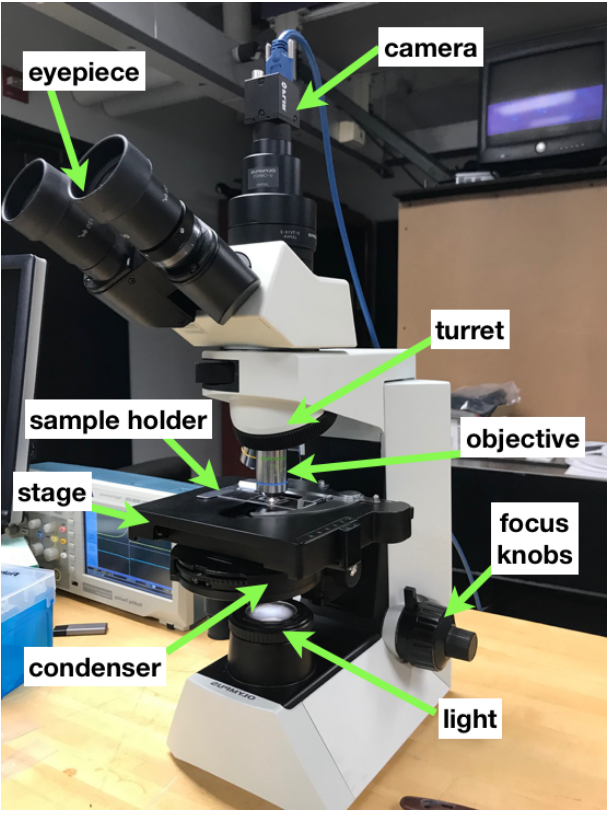
\includegraphics[ width = 0.8 \linewidth ]{microscope.PNG}
    \caption{Image of the microscope with its features labeled}
    \label{fig:microscope}
\end{figure}
It should be noted that the condenser is used to focus the light coming from the light source into a cone. If properly aligned, then the cone narrows to a point at the sample, and then expands back into a cone of light that enters the objective an angle (i.e. the cone angle) that matches numerical aperture (or acceptance angle) for said objective. Furthermore, adjusting the position of the condenser, the diameter of the iris, and brightness of the light source are all vital towards getting the best image possible.

\subsection{Camera and Programs}
For video recording, we used a CMOS camera (model FLIR Blackfly S BFS-U3-32S4M). As discussed in the microscope section, the camera is coupled to the microscope and is also connected to the computer via USB. As for actually seeing the output of the camera, the \texttt{Spinview} application is needed, and the application allows for us to take both images and videos. Some of the key settings that \texttt{Spinview} provides are the following:
\begin{itemize}
    \item Options to adjust the exposure time and frame rate;
    \item Options to adjust the gamma correction to the output of the camera; and
    \item Ability to record videos as a batch of TIFF images.
\end{itemize}
The other programs that we used were \texttt{ImageJ} and \texttt{TrackPy}; these two programs allowed for us to analyze the data and calculate the diffusion constant (as well as $k_{B}$).

\section{Measurements and Data Analysis}

\subsection{Data Collection}
We note that the following procedure was done for all five colloidal samples. 

\subsubsection{Preparing the Colloidal Sample}
In order to view the colloidal sample under the microscope, we first had to dilute it. We decided to dilute each sample 15 to 1 water to solution (where we used a pipette to get the measurements close to exact), and made sure to vortex the colloidal sample well before mixing it in with water in a tube (that could be closed to prevent the water in the sample from evaporating too much). We then vortexed the contents of the tube to form a diluted homogeneous mixture of the colloidal sample. From here, we prepared this mixture onto the microscope slide, and there were two ways that we did this.

The first method involved taping a small strip of double-sided tape on a microscope slide. We then used a knife to cut a small rectangular hole in the tape -- small enough so that the coverslip covers the entire hole. We then pipetted a small amount of our diluted mixture (about $10 \ \si{\mu L}$) into the rectangular hole making sure to not overfill it. We then used tweezers to place a coverslip over the hole and gently pressed the coverslip down to ensure a tight seal with the double-sided tape.

The second method was much simpler; it consisted of dipping a capillary tube into the tube that contained our diluted mixture. Once enough of the mixture filled the tube, we then used a wipe to remove any residue on the outside of the tube. Finally, we taped the capillary tube onto the microscope slide. 

It should be noted that we got the capillary tubes about a week and a half into the lab, so we prepared the microscope slides using both methods. We re-prepared the slides from our prepared mixtures each day if needed, because the slides from the previous day had dried between lab days. Also, we remade the diluted mixtures if they were a few days old in case the dilution ratio changed at all from the water evaporating.

\subsubsection{Using \texttt{Spinview} to Capture Videos}
Once the colloidal sample was prepared, we viewed it under a microscope using the 40x objective. Again, the program that we used to see the output of the camera was \texttt{Spinview}. We made sure to adjust the focus, the gamma correction, the exposure time, the position of the condenser, the diameter of the iris, and the brightness of the light source so that the image is as clear as it can get; having a clear image is vital for \texttt{ImageJ} and \texttt{TrackPy} to work correctly. Once we were satisfied with the image quality, we then set the frame rate of the camera output to be 10 frames per second and recorded a 300 frame video (more accurately, we captured 300 TIFF image files).

\subsection{Data Analysis}

\subsubsection{Using \texttt{ImageJ} and \texttt{TrackPy} to Calculate the Diffusion Coefficient}
We can now hand the video over to \texttt{TrackPy}, which will help us calculate the diffusion constant. We followed the procedure outlined in the walkthrough section of the \texttt{TrackPy} documentation, and the full details of using the program can be found there \cite{trackpy}. In short, though, we use \texttt{TrackPy} to identify the particles in the video. On top of that, \texttt{TrackPy} tracks and records the $x$ and $y$ displacement of each particle that it identified. However, these displacements are given in units of pixels, and we need to convert it into microns. 

This is where \texttt{ImageJ} is helpful. We are able to convert from pixels to microns using a stage micrometer that has rulings inscribed on it in increments of $0.1 \ \si{mm}$ and $0.01 \ \si{mm}$. Since we only used the 40x objective, it suffices that we find the micron-pixel conversion rate under the 40x objective. Figure \ref{fig:scale} shows the image that we captured.
\begin{figure}[ht]
    \centering
    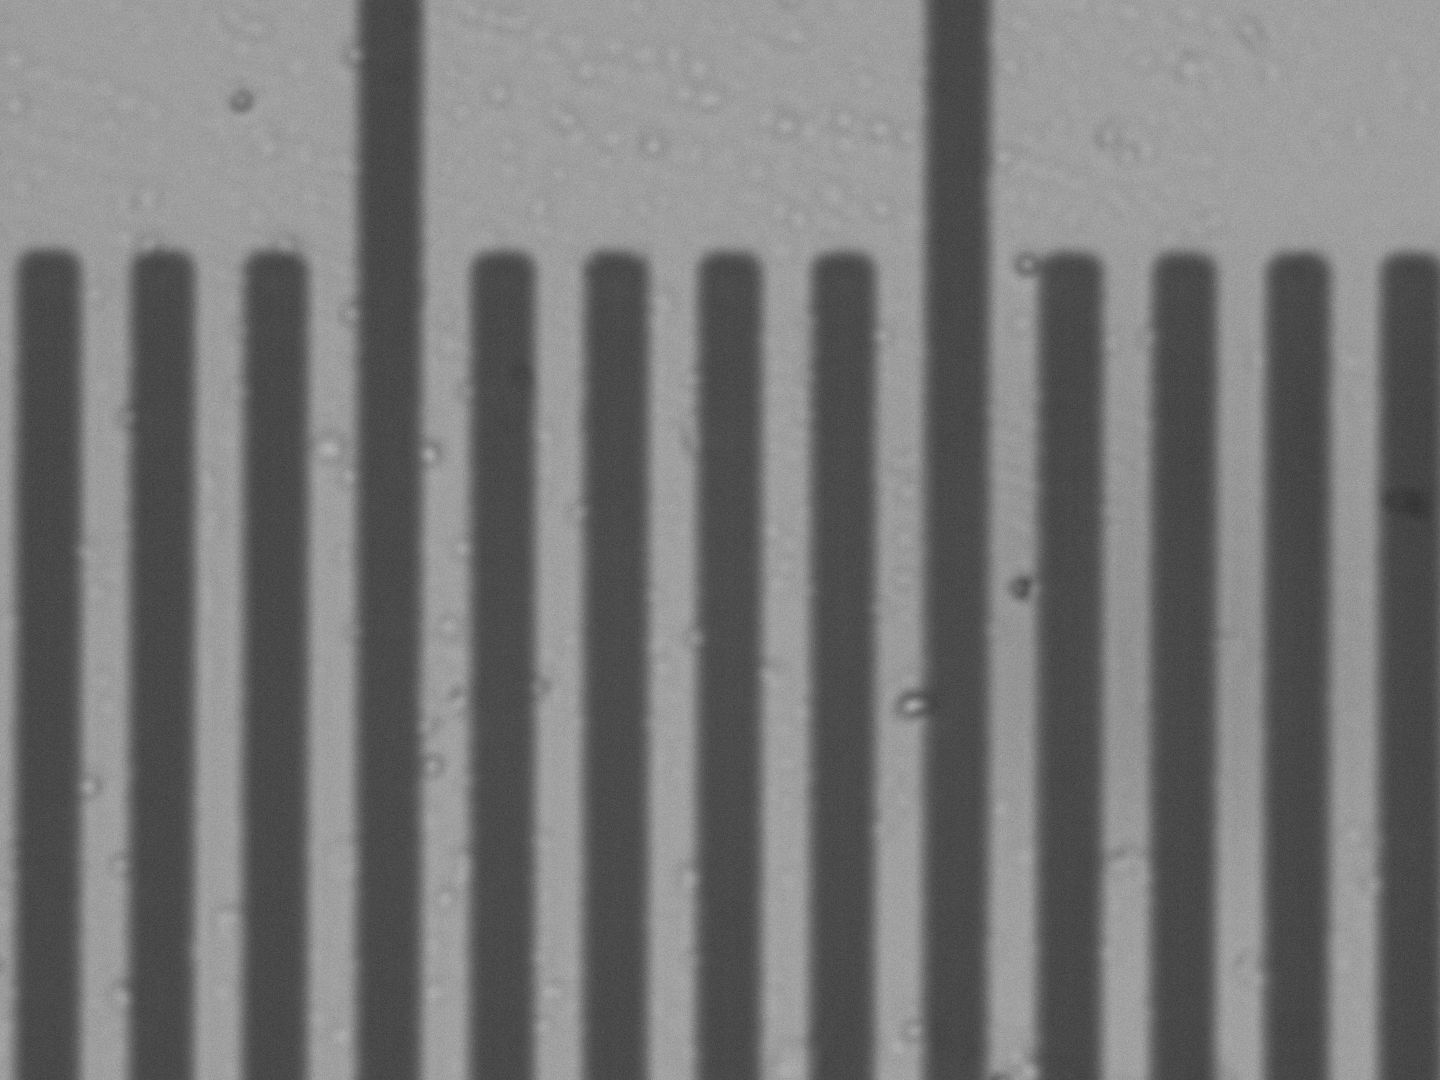
\includegraphics[ width = 0.8 \linewidth ]{Scale_x40.png}
    \caption{Image of the stage micrometer under 40x objective}
    \label{fig:scale}
\end{figure}
We then exported this image to \texttt{ImageJ} and used the program to find how many pixels were needed to get a length of $0.1 \ \si{mm}$. In our case, we got a conversion of 0.0880 microns per pixel. 

We also note that we used \texttt{ImageJ} to find the approximate diameter (in pixels) of a particle in our diluted mixture. This information was used to tell \texttt{TrackPy} to identify particles of approximately this diameter.

Now that we have the micron-pixel conversion, we are able to extract/calculate the diffusion coefficient from the displacement data that we gathered. We utilize method 2 as described in the section on measuring the diffusion constant. As already noted in that section, we use \texttt{TrackPy} to calcluate the EMSD of all the particles and graph this result out over time. It should be noted that \texttt{TrackPy} records the net displacement as well as the displacement along the $x$- and $y$-axes. We only need the displacement data along the $x$-axis (or the $y$-axis, whichever gives us a better linear fit -- however, we should expect the linear fit from either axes to give us the same result) since our model only accounts for one dimension. It should be noted that we can easily extend it to two, if we want, by noting that $\langle x^{2} \rangle = \langle y^{2} \rangle$. Thus:
\begin{equation}
    \langle r^{2} \rangle 
    =
    \langle x^{2} \rangle + \langle y^{2} \rangle
    =
    2 \langle x^{2} \rangle
    \implies 
    \langle r^{2} \rangle 
    =
    4 D t
    \label{eq:da-1}
\end{equation}
We then perform a linear fit of the EMSD vs. time graph, whose slope gives us $2 D$ (where $D$ is the diffusion constant). From this, we can immediately get the diffusion constant, which then immediately gives us $k_{B}$. Figure \ref{fig:trajectory} is an example of what \texttt{TrackPy}'s particle-tracking outputs, and Figures \ref{fig:position} and \ref{fig:displacement} are the corresponding plots of the particle's trajectories in position space as well as the EMSD over time. As expected, we do indeed see in Figure \ref{fig:displacement} that the relationship between EMSD and time is linear.

\begin{figure}
    \centering
    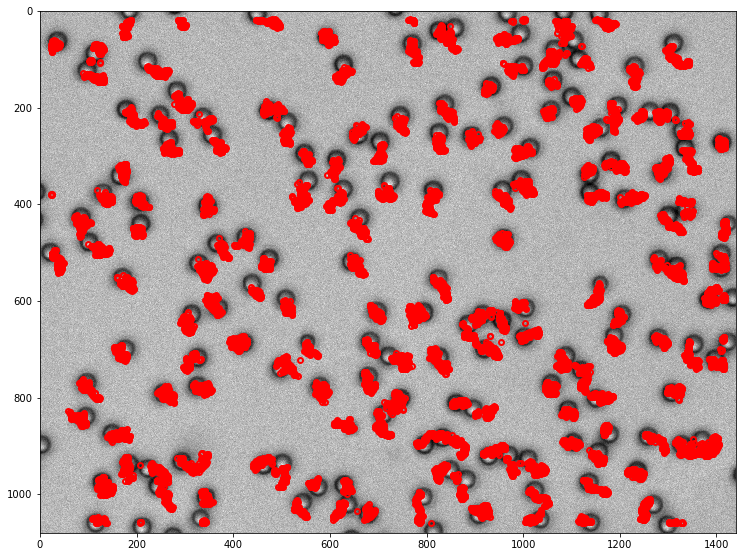
\includegraphics[ width = 0.8 \linewidth ]{trackpy_trajectory.png}
    \caption{Recorded trajectories of particles done by \texttt{TrackPy}}
    \label{fig:trajectory}
\end{figure}

\begin{figure}
    \centering
    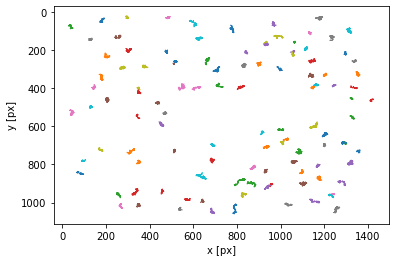
\includegraphics[ width = 0.8 \linewidth ]{trackpy_trajectory_xy.png}
    \caption{Plot of recorded trajectories of particles in the $xy$-plane}
    \label{fig:position}
\end{figure}

\begin{figure}
    \centering
    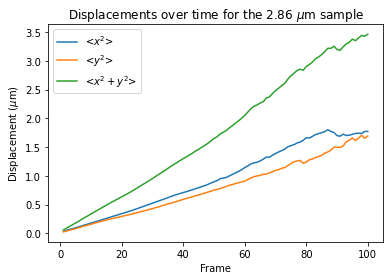
\includegraphics[ width = 0.8 \linewidth ]{trackpy_displacement.png}
    \caption{Plot of EMSD vs. Time}
    \label{fig:displacement}
\end{figure}

\subsubsection{Extensions}
We now perform three extensions to our existing procedure: varying the particle density of our mixture, varying the frame rate of the camera output, and varying the track length used by our python notebook to calculate our final results. For the first two extensions, we work with the colloid sample that contains particles with $1 \ \si{\mu m}$ diameter, and for the track length extension we include trials with the $2.12 \ \si{\mu m}$ sample. 

For the extension that involves varying the particle density of our mixture, we repeat the procedure already described, but with the sample now being diluted 5 to 1 as well as 30 to 1 ratios of water to solution. 

For the extension that involves changing the frame rate of the camera output, we again repeat the procedure, but with a frame rate of 5 as well as 15.

For the extension that involves changing the track length, we use trials which resulted in basically accurate measurements of $k_B$ (15 to 1 dilutions of $1 \ \si{\mu m}$ and $2.12 \ \si{\mu m}$ samples) and re-ran our python notebook, now with the track length setting varied to be shorter and longer than the initial setting. This changed the cutoff length of the track of the particles located by \texttt{TrackPy} for inclusion in the final calculation of our constants--a higher track length is a more stringent requirement, so fewer points were included in the final calculation, and vice versa. 

Again, the main goal of these extensions is to see how varying these three parameters will affect the diffusion constant and result for $k_B$ as well as how it might change the way we analyze our data.

% \subsection{Data Analysis}
% $T = 295.15 \si{K}$

\subsection{Results}
Our results of our main experiment are shown in Table I. As described in the caption of that table, these results were obtained from 15:1 water to solution samples, captured with a frame rate of 10. Different track lengths were used for each size, but the setting was consistent for all trials of the same size sphere. The quoted uncertainty is obtained from a standard deviation of our results over several trials. The \SI{}{\percent} Error column is the \SI{}{\percent} difference between our experimental result for $k_B$, and the established value of $k_B = 1.3806\times10^{-23}$.

\begin{table}[H]
\centering
% \caption{Results for diffusion constant $D$ and Boltzmann constant $k_B$ for various polystyrene sphere sizes.} 
\label{tab:results}
% \renewcommand{\arraystretch}{1.3}
\begin{tabular}{||l|c|c|c|c||}
 \hline
 \bf Sphere & \textbf{$D$} & \bf $k_B$ & Error & $\sigma$ \\
    \bf Size ($\si{\mu m}$) &   &  &  \SI{}{\percent} & \\
 \hline
 \bf $0.52 \si{\mu m}$ & $0.35 \pm 0.01$ & $(0.56 \pm 0.02) \times10^{-23}$ & $6.0$ & $>10\sigma$ \\
 \bf $0.76 \si{\mu m}$ & $0.54 \pm 0.04$ & $(1.25 \pm 0.08) \times10^{-23}$ & $1.0$ & $2\sigma$\\
 \bf $1 \si{\mu m}$ & $0.43 \pm 0.03$ & $(1.30 \pm 0.10) \times10^{-23}$ & $0.6$ & $1\sigma$\\
 \bf $2.12 \si{\mu m}$ & $0.23 \pm 0.01$ & $(1.46 \pm 0.05) \times10^{-23}$ & $0.5$ & $2\sigma$\\
 \bf $2.86 \si{\mu m}$ & $0.25 \pm 0.05$ & $(2.13 \pm 0.41) \times10^{-23}$ & $5.5$ & $2\sigma$\\
%  \bf $87\mathrm{a}_{\mathrm{F}': 1, 2}$ & $0.1549 \pm 0.0023$ & $0.157$ \\
%  \bf $87\mathrm{b}_{\mathrm{F}': 1, 2}$ & $0.1562 \pm 0.0024$ & $0.157$ \\
%  \bf $87\mathrm{b}_{\mathrm{F}': 2, 3}$ & $0.2695 \pm 0.0055$ & $0.287$ \\
 \hline
\end{tabular}
\caption{Results for diffusion constant $D$ and Boltzmann constant $k_B$ for various polystyrene sphere sizes. Each of these results is a mean value based on several trials. Each was obtained from measurement and analysis of a 15:1 water to solution sample, captured with a frame rate of 10. The track length varied across different sized samples, but was consistent within trials for the same size sample.}
\end{table}

\subsubsection{Particle Density Extension}
Results of our first extension, comparing results across different dilutions of our $1 \si{\mu m}$ sample, are shown in Table II. 

\begin{table}[H]
\centering
% \caption{Results for diffusion constant $D$ and Boltzmann constant $k_B$ for various polystyrene sphere sizes.} 
\label{tab:density}
% \renewcommand{\arraystretch}{1.3}
\begin{tabular}{||l|c|c|c|c||}
 \hline
 \bf Dilution & \textbf{$D$} & \bf $k_B$ & Error & $\sigma$\\
    \bf  &   &  & \SI{}{\percent} &\\
 \hline
 \bf $5:1$ & $0.46 \pm 0.02$ & $(1.39 \pm 0.07) \times10^{-23}$ & $0.1$ & $1\sigma$\\
 \bf $15:1$ & $0.43 \pm 0.03$ & $(1.30 \pm 0.10) \times10^{-23}$ & $0.6$ & $1\sigma$\\
 \bf $30:1$ & $0.45 \pm 0.01$ & $(1.38 \pm 0.03) \times10^{-23}$ & $0.0$ & $1\sigma$\\
%  \bf $2.12 \si{\mu m}$ & $0.225 \pm 0.007$ & $(1.455 \pm 0.050) \times10^{-23}$ \\
%  \bf $2.86 \si{\mu m}$ & $0.245 \pm 0.047$ & $(2.133 \pm 0.409) \times10^{-23}$ \\
%  \bf $87\mathrm{a}_{\mathrm{F}': 1, 2}$ & $0.1549 \pm 0.0023$ & $0.157$ \\
%  \bf $87\mathrm{b}_{\mathrm{F}': 1, 2}$ & $0.1562 \pm 0.0024$ & $0.157$ \\
%  \bf $87\mathrm{b}_{\mathrm{F}': 2, 3}$ & $0.2695 \pm 0.0055$ & $0.287$ \\
 \hline
\end{tabular}
\caption{Results for diffusion constant $D$ and Boltzmann constant $k_B$ for samples of various dilutions. Each of these results is a mean value based on several trials. Each was obtained from measurement and analysis of a $1 \si{\mu m}$ sample, captured with a frame rate of 10 and a track length consistent across measurements from the same dilution.}
\end{table}

\subsubsection{Frame Rate Extension}
Results of our second extension, comparing results across different frame rates, are shown in Table III. 

\begin{table}[H]
\centering
% \caption{Results for diffusion constant $D$ and Boltzmann constant $k_B$ for various polystyrene sphere sizes.} 
\label{tab:framerate}
% \renewcommand{\arraystretch}{1.3}
\begin{tabular}{||l|l|c|c|c|c||}
 \hline
 \bf Dilution & \bf Frame & \textbf{$D$} & \bf $k_B$ & Error & $\sigma$\\
    \bf  & \bf Rate & &  & \SI{}{\percent} &  \\
    \bf & (fps) & & & & \\
 \hline
 \bf $15:1$ & $5$ & $0.41 \pm 0.03$ & $(1.25 \pm 0.09) \times10^{-23}$ & $1.0$ & $2\sigma$\\
 \bf $15:1$ & $10$ & $0.43 \pm 0.03$ & $(1.30 \pm 0.10) \times10^{-23}$ & $0.6$ & $1\sigma$\\
 \bf $15:1$ & $15$ & $0.28 \pm 0.01$ & $(0.85 \pm 0.03) \times10^{-23}$ & $3.8$ & $>10\sigma$\\
 \hline
 \bf $30:1$ & $5$ & $0.45 \pm 0.01$ & $(1.38 \pm 0.03) \times10^{-23}$ & $0.0$ & $1\sigma$\\
 \bf $30:1$ & $10$ & $0.45 \pm 0.01$ & $(1.38 \pm 0.03) \times10^{-23}$ & $0.0$ & $1\sigma$\\
 \bf $30:1$ & $15$ & $0.46 \pm 0.02$ & $(1.40 \pm 0.05) \times10^{-23}$ & $0.1$ & $1\sigma$\\
%  \bf $87\mathrm{a}_{\mathrm{F}': 1, 2}$ & $0.1549 \pm 0.0023$ & $0.157$ \\
%  \bf $87\mathrm{b}_{\mathrm{F}': 1, 2}$ & $0.1562 \pm 0.0024$ & $0.157$ \\
%  \bf $87\mathrm{b}_{\mathrm{F}': 2, 3}$ & $0.2695 \pm 0.0055$ & $0.287$ \\
 \hline
\end{tabular}
\caption{Results for diffusion constant $D$ and Boltzmann constant $k_B$ for different frame rates; conducted on both $15:1$ and $30:1$ dilutions of the $1 \si{\mu m}$ solution. Each of these results is a mean value based on several trials.}
\end{table}

\subsubsection{Track Lengths Extension}
Results of our third extension, comparing results across different track lengths, are shown in Table IV. 

\begin{table}[H]
\centering
% \caption{Results for diffusion constant $D$ and Boltzmann constant $k_B$ for various polystyrene sphere sizes.} 
\label{tab:tracklength}
% \renewcommand{\arraystretch}{1.3}
\begin{tabular}{||l|l|c|c|c|c||}
 \hline
 \bf Sphere & \bf Track & \textbf{$D$} & \bf $k_B$ & Error & $\sigma$\\
    \bf Size ($\si{\mu m}$) & \bf Length  & & & \SI{}{\percent} &  \\
 \hline
 \bf $1 \si{\mu m}$ & $5$ & $0.42 \pm 0.03$ & $(1.29 \pm 0.10) \times10^{-23}$ & $0.6$ & $1\sigma$\\
 \bf $1 \si{\mu m}$ & $15$ & $0.43 \pm 0.03$ & $(1.30 \pm 0.10) \times10^{-23}$ & $0.6$ & $1\sigma$\\
 \bf $1 \si{\mu m}$ & $50$ & $0.20 \pm 0.09$ & $(0.60 \pm 0.26) \times10^{-23}$ & $5.7$ & $3\sigma$\\
 \hline
 \bf $2.12 \si{\mu m}$ & $5$ & $0.23 \pm 0.01$ & $(1.48 \pm 0.04) \times10^{-23}$ & $0.7$ & $3\sigma$\\
 \bf $2.12 \si{\mu m}$ & $25$ & $0.23 \pm 0.01$ & $(1.45 \pm 0.05) \times10^{-23}$ & $0.5$ & $2\sigma$\\
 \bf $2.12 \si{\mu m}$ & $50$ & $0.22 \pm 0.001$ & $(1.41 \pm 0.01) \times10^{-23}$ & $0.2$ & $5\sigma$\\
 \bf $2.12 \si{\mu m}$ & $115$ & $0.15 \pm 0.04$ & $(0.99 \pm 0.28) \times10^{-23}$ & $2.8$ & $2\sigma$\\
%  \bf $87\mathrm{a}_{\mathrm{F}': 1, 2}$ & $0.1549 \pm 0.0023$ & $0.157$ \\
%  \bf $87\mathrm{b}_{\mathrm{F}': 1, 2}$ & $0.1562 \pm 0.0024$ & $0.157$ \\
%  \bf $87\mathrm{b}_{\mathrm{F}': 2, 3}$ & $0.2695 \pm 0.0055$ & $0.287$ \\
 \hline
\end{tabular}
\caption{Results for diffusion constant $D$ and Boltzmann constant $k_B$ for various track lengths. Each of these results is a mean value based on several trials. Each was obtained from measurement and analysis of a 15:1 water to solution sample, captured with a frame rate of 10.}
\end{table}



\section{Discussion}

The majority of our results are within $2\sigma$ of the established $k_B$ value we expect to find from theory. The exception to this from our main experimental results is the result from the $0.52 \si{\mu m}$ sample. Of all of our measurements, this is the one with the greatest percent error, but it also has one of the smallest uncertainties. This means that our measurements were consistently yielding small diffusion coefficients ($D$) and thus small values for $k_B$.

From our particle density extension, we find that with a $1 \si{\mu m}$ sample, we are able to recover results within $1\sigma$ to what we expect for $k_B$ for all three particle dilutions. There is no recognizable trend that we can identify regarding how $D$ or $k_B$ scale with particle density in our sample. 

From our frame rate extension, we find that the effects of the frame rate also depend on the dilution of the sample. For the $15:1$ dilution, decreasing the frame rate to $5$ pushed our result further from the expected value, and increasing the frame rate to $15$ significantly decreased our measured $D$ and caused our $k_B$ value to be $>10\sigma$ from the expected value. However, varying the frame rate in the $30:1$ dilution did not have similarly significant results: we were able to recover $k_B$ to within \SI{0.1}{\percent} for each frame rate. This may be because the \texttt{TrackPy} tracking finds it harder to associate particles in one frame with the same particle in the neighboring frames when there are twice as many particles present in the sample; the $30:1$ dilution makes it easier to identify and track unique particles, even when greater or fewer frames are captured per second. 

From our track lengths extension, we find that our best results come from the middling track lengths that we chose for our initial results. For the $1 \si{\mu m}$ sample, shortening the track length did not change our results much, but lengthening it to $50$ (where only about $5$ particles were being tracked in each trial) nearly tripled our uncertainty, and caused our measured $D$ and $k_B$ to be much lower than expected. For the $2.12 \si{\mu m}$ sample, the percent error for track lengths $5$ through $50$ is not very high, but the uncertainties are likely being underestimated; lowering the track length potentially includes spurious tracks, and increasing it causes our measurement to be based on fewer "trials" (as each particle tracked can count as a "trial" of measuring the mean-squared displacement of a particle under Brownian motion). For the $2.12 \si{\mu m}$ sample, a track length of $50$ still retained about $52$ particles for each trial; the track length of $115$ yields the result for $k_B$ that is furthest from expected, as each trial was only retaining the tracking of about $5$ particles. 

One possible source of error could have come from our sample being exposed to the light source for a long period of time (e.g. 30 minutes).
It should be noted that we assumed the temperature of the fluid to be constant when we calculated both the diffusion and Boltzmann constant. However, might not be the case when we did the lab since the light source within the apparatus could have heated up our samples. We would expect the change in temperature to be negligible since water requires quite a lot of energy to heat it up. However, we note that the high intensity of our light source along with the time that the sample is exposed to it (up to 30 minutes at the most) could result in a non-negligible change in temperature of our sample -- especially with the sample being a small amount of water (around $10 \ \si{\mu L}$). Thus, because both the diffusion and Boltzmann constant depends on temperature, a change in temperature would result in the value of the two constants to change as well.

We should also note that we had to estimate what the temperature of each sample would be. As noted in the Data Analysis section, we took each sample to be the temperature of the lab room, which we also had to estimate as well. Thus, us not knowing the exact temperature of the sample to begin with could have contributed to a noticeable error with our calculation of the two constants.

Another possible source of error could be from the the particles undergoing non-random drift. In some runs, we found this non-random drift to be heavily present (e.g. the trajectories of all particles in one run were a straight line down). Oone possible cause of this drift could be a non-level microscope surface; though the particles are suspended in liquid and very small, we can't rule out the possible effect of gravity on the system. Another possible source for this non-random drift could be from the sample leaking from the rectangular hole. We think that when leakage is present, the particles near the edges of the rectangular hole would want to move with the leakage -- that is, the particles would be subject to a non-Brownian force to move in a particular direction.

This is where we note that we manually made the rectangular hole for each sample. The size of the hole therefore varied while the amount that we put in stayed about the same (again, around $10 \ \si{\mu L}$), and this could result in some leakage to occur in some samples if the hole was made too small. 

Furthermore, if the hole is too large, then there would not be enough of the sample to fill the hole; this resulted in air bubbles to be present in the sample. This could be another possible source for the non-random drift. In some cases, the air bubbles were much larger than the particles, and the movement of these air bubbles could displace them such that their trajectories are no longer random. 

Finally, one other possible source of error would be from how we used \texttt{TrackPy}. To expand on this, we had to play around with a lot of parameters to make sure that \texttt{TrackPy} was tracking actual particles (e.g. \texttt{TrackPy} might mistake a darker region to be a particle) and that the trajectories for those particles were not too short (e.g. we wanted to omit trajectories that only lasted a couple frames since it could result skew our data). We note that changing parameters would almost certainly change the values that we would get for the diffusion and Boltzmann constant; most of the time, these changes would be small, but there were instances where the change was drastic. Thus, the values that we calculated from \texttt{TrackPy} might not be the most accurate that they could be. However, the more comfortable we got with using \texttt{TrackPy} (i.e. understanding what each of the parameters did), we feel that we mostly utilized \texttt{TrackPy} correctly and find that the error from our use of \texttt{TrackPy} is likely not a significant source of error.

\section{Conclusion}

In this lab, we were generally successful in experimentally measuring the Boltzmann constant $k_B$ by observing and analyzing the Brownian motion of small polystyrene spheres in water. The majority of our results were within $2\sigma$ of the established and expected value of $k_B$. We found that, generally, our results were closest to the expected value when using a $1 \si{\mu m}$ sample at any dilution, with a frame rate of 10 and a track length of 15 or shorter. This finding is due to the limitations of our apparatus and software, which were best attuned to capture and track spheres of that size.    

One possible improvement would be to use capillary tubes for all samples. This would almost certainly remove our issues with leakages or air bubbles, which in turn would mitigate any non-random drift.

Another improvement would be taking exact temperatures of the samples prior to capturing our data, so that we could take into account possible shifts in the base sample temperature over the several days of the experiment. Indeed it would be even better to quantify the possible temperature change due to the light source that may occur while collecting data; this may be done by taking the temperature of the sample after taking our measurements, but this would be made difficult by the small amount of sample on each slide.

Our experimental results could also be improved with some improvements to \texttt{TrackPy}, including automating the ideal particle size based on the .tiff images we supplied. We used \texttt{ImageJ} to make an educated guess of what particle size we should tell \texttt{TrackPy} to track, but some adjustments needed to be made to procure good results in some cases. We largely based our \texttt{TrackPy} settings on by-eye evaluations of the plots shown in Figures \ref{fig:trajectory}, \ref{fig:position} and \ref{fig:displacement}, but accuracy could be improved by the inclusion of some automated evaluations of these fits in the \texttt{TrackPy} program. 

We believe that extensions of the lab to allow for more data collection would also help improve our results, especially for the particle sizes for which our results were far from the expected value (namely $0.52 \si{\mu m}$ and $2.86 \si{\mu m}$). Though our apparatus and analysis software was obviously not ideal to obtain results from these samples, we believe that better results could have been obtained by attempting many different setups--essentially, by performing all of our extensions on all of our samples, instead of just a few. We may have been able to find different dilutions, frame rates, or track lengths which yielded better results for these samples, given more time. 

\section{Figure References}
Figure \ref{fig:microscope} can be found in the Brownian motion handout on our Canvas page.

\bibliographystyle{unsrt}
\bibliography{References}

\end{document}